\section{Numerical Experiments}
\label{sec:experiments}

We evaluate WAIT and Nested WAIT on synthetic Poisson workloads (Section~\ref{sec:exp_synthetic}) and a real workload sampled from lmsys-chat-1m (Section~\ref{sec:exp_real}). We benchmark against vLLM~\citep{kwon2023efficient} and Sarathi~\citep{agrawal2023sarathi}, both greedy FCFS-based serving policies in our experiments; Sarathi differs by splitting long prefills into chunks that can be interleaved with decode work. We use Vidur~\citep{agrawal2024vidur} as the discrete-event simulator, configured for a single NVIDIA A100~80\,GB serving Llama-2-7B. Appendix~\ref{app:additional_experiments} validates Vidur's iteration-time predictions against physical A100 measurements over the profiled range and at an extrapolation point \(B=256\), and also reports end-to-end real-GPU runs of WAIT and Nested WAIT. The workloads below stress decode-side KV-cache growth, the regime targeted by the linear iteration-time approximation in Section~\ref{sec:model}.

With exogenous arrivals at rate $\lambda$, policies in the stable region complete requests at the offered load, so completion-rate differences appear only when a policy approaches or exceeds the arrival rates it can sustain. We use mean end-to-end latency as the primary delay metric in the numerical study. The main figures plot this latency against $\lambda$ and pair it with effective completion rate, which shows whether a policy continues to handle the offered load or instead saturates because of overload or eviction-induced restarts. Each latency point averages $10$ independent simulation replications. Within each replication, latency is averaged over a central measurement window after the initial transient, using the same window across policies. We use $\hat{\lambda}^*$ to mark the observed transition point from the near-overloaded to the overloaded regime: it is the largest reported rate at which latency remains controlled and effective completion rate still tracks the offered load. Above that range, completion rate saturates or declines because the policy suffers overload or eviction-induced restarts, and the paired completion-rate panel records this loss of sustainable service.

\textbf{Hardware.} All experiments use Vidur to simulate a single NVIDIA A100~80\,GB serving Llama-2-7B~\citep{nvidia-a100-specs,huggingface-llama2-docs}. A FP16 KV-cache token for this model occupies \(2\) (key/value) \(\times 32\) layers \(\times 32\) KV heads \(\times 128\) head dimension \(\times 2\) bytes, or \(524{,}288\) bytes (\(0.5\) MiB)~\citep{huggingface-kv-cache-basics}. After model weights and the baseline \(1\%\) memory margin, the baseline-memory runs use a KV-cache cap of approximately \(1.37\times 10^5\) tokens. If resident KV cache exceeds the cap, the server evicts and restarts in-progress requests. The iteration-time model is Equation~\eqref{eq:time_consump}; its A100 validation is reported in Appendix~\ref{app:gpu_validation}.

\textbf{Baseline configurations (vLLM, Sarathi).} Both baselines use their default Vidur configurations and greedily admit arrivals in FCFS order. They also use the same local capacity-reservation rule: before admitting a new request, the scheduler requires a small memory buffer ($1\%$ of KV-cache capacity) to remain unused. This rule protects against admitting a request when the server is already essentially full, but it is not a dynamic limit on the total number of jobs in service. Once admitted requests continue decoding, their KV caches can still grow beyond the available capacity, in which case the scheduler evicts and restarts an in-progress request. The difference between the baselines is in how prefill is batched. vLLM processes a newly admitted request's full prefill in one iteration. Sarathi bounds the prefill work per iteration to chunks of at most $512$ tokens, allowing partial prefills to be interleaved with decode iterations. This chunked-prefill rule reduces head-of-line blocking from long prefills, but it does not control the cumulative decode-side population. Thus neither baseline enforces the load-balancing threshold used by WAIT.

\textbf{WAIT and Nested WAIT settings.} In the experiments below, the main parameter for WAIT and Nested WAIT is a system-wide batch-size cap $\mathrm{tl}$, calibrated on the common finite parameter grid \(\{20,30,\ldots,300\}\). The cap controls how many requests can be served concurrently across prefill and decode stages, but it is not itself one of the per-stage scheduling thresholds. In a single-type WAIT run, once $\mathrm{tl}$ is chosen, the integer per-stage thresholds are computed by distributing this cap across the prefill/decode stages of the workload. For Nested WAIT, we first partition the decode horizon into \(L\) ordered segments. Let \(\Delta l_k'\) be the number of decode stages in segment \(k\), and let \(\lambda_k'\) be the arrival rate of requests whose final decode length lies in that segment. A request reaches segment \(k{+}1\) only if its decode length exceeds the end of segment \(k\), so the continuation probability from segment \(k\) to segment \(k{+}1\) is \(p_k=(\sum_{r=k+1}^L\lambda_r')/(\sum_{r=k}^L\lambda_r')\). Given the margin parameter \(\eta\), we set \(q_k=\min\{p_k+\eta,0.99\}\). Once \(\mathrm{tl}\), \(L\), and \(\eta\) are fixed, the real-valued per-stage thresholds are computed as \(n_k=n_1\prod_{r<k}q_r\), where \(n_1\) solves \(\sum_{k=1}^L \Delta l_k' n_k=\mathrm{tl}\). The segment-level cap \(B_k=\Delta l_k'n_k\) is then rounded to an integer and spread as evenly as possible across the stages in that segment. Thus, \(\mathrm{tl}\) fixes the overall threshold scale, while \(L\), \(\eta\), and the continuation probabilities determine how that scale is allocated across decode segments. The workload-specific subsections describe the corresponding threshold and segment design. The calibration uses only the workload distribution and the offered arrival rate; the online scheduler does not use realized future arrivals or unrevealed final output lengths. Under the baseline settings used for the arrival-rate figures, WAIT and Nested WAIT do not trigger eviction.


\subsection{Synthetic Workloads}
\label{sec:exp_synthetic}

We consider three synthetic Poisson workloads. The single-type workload \texttt{p512d20} has prefill length $512$ and decode length $20$, isolating the effect of WAIT's threshold mechanism (Algorithm~\ref{alg:wait}). The two-type workload $(0.7\,\texttt{p512d20},\,0.3\,\texttt{p512d50})$, meaning that each arrival is \texttt{p512d20} with probability $0.7$ and \texttt{p512d50} with probability $0.3$, tests the segment design of Nested WAIT (Algorithm~\ref{alg:nested_wait}) on prompts that share the prefill profile but differ in decode length. The long-decode workload \texttt{p512d1000} keeps the same prefill length but increases the decode length to $1000$, allowing us to examine the same threshold mechanism when KV cache growth is much more pronounced.

\paragraph{Single-type workload (WAIT).}
For this workload, WAIT converts the selected $\mathrm{tl}$ into the corresponding per-stage limits. Figure~\ref{fig:single_type_rate} shows mean end-to-end latency (left, on a stretched-symlog scale that expands the stable region) and effective completion rate (right), i.e., completed requests per second net of eviction-induced restarts, versus arrival rate $\lambda$. Because all requests are homogeneous, this workload highlights the effect of threshold-based admission without the additional segment structure used in Nested WAIT. WAIT keeps latency controlled up to $\lambda \approx 23$, whereas Sarathi and vLLM lose stability near $\lambda \approx 22$ and $\lambda \approx 19$, respectively. At low load the three policies are close, but the gap widens rapidly as $\lambda$ approaches the boundary: WAIT attains the smallest mean latency at every tested rate in $\lambda \in \{12, \dots, 24\}$, with the gap to Sarathi growing from ${\sim}2\%$ at $\lambda = 12$ to over $70\%$ at $\lambda = 23$. Because there is only one request type, the gain does not come from type separation; it comes from threshold-based admission itself, which keeps the batch composition closer to the balanced prefill/decode composition and delays the onset of instability. The right panel shows the same insight in completion-rate terms: WAIT follows the ideal $\lambda$-line up to a higher arrival rate than Sarathi and vLLM.

\begin{figure}[htbp]
    \centering
    
\includegraphics[width=0.76\textwidth]{Experiments_pdf/figure_B_single_type.pdf}
    \caption{Single-type workload (\texttt{p512d20}): mean end-to-end latency (left) and effective completion rate (right) versus $\lambda$. Arrows mark the transition from near-overloaded to overloaded operation; the dotted line is the ideal completion rate \(\lambda\).}
    \label{fig:single_type_rate}
\end{figure}

\paragraph{Two-type workload (Nested WAIT).}
For the two-type workload, Nested WAIT uses the same system-wide batch-size cap $\mathrm{tl}$ and two decode-stage segments, $1$--$20$ and $21$--$50$. The second segment receives the prompts that survive the first $20$ decode stages, so its continuation ratio is $0.3$. Thus the allocation rule above gives real-valued per-stage thresholds in the ratio $n_2/n_1=0.3$ and solves $20n_1+30n_2=\mathrm{tl}$ before rounding the corresponding segment-level caps to integers; for example, $\mathrm{tl}=30$ gives segment-level caps approximately $21$ and $9$. Figure~\ref{fig:multi_type_rate} shows the same comparison for the two-type workload $(0.7\,\texttt{p512d20},\,0.3\,\texttt{p512d50})$. The stability ordering is again vLLM first ($\hat{\lambda}^* \approx 18$), Sarathi second ($\hat{\lambda}^* \approx 21$), and Nested WAIT last ($\hat{\lambda}^* \approx 22$). Nested WAIT attains the lowest mean latency over these tested rates, with the gap to Sarathi growing from ${\sim}6\%$ at low load to over $40\%$ near the boundary. The mechanism also differs from the single-type case. Here the two request classes have the same prefill length and differ only in decode length, so the main source of congestion is the accumulation of the long-decode minority in later decode stages. Nested WAIT's segment thresholds keep that downstream inventory from expanding too far, which prevents those delays from propagating to the short-decode majority. The resulting gain is therefore not only at entry: by controlling downstream buildup, Nested WAIT preserves low latency for the short jobs and enlarges the stable operating region beyond what a single global cap can achieve.

\begin{figure}[htbp]
    \centering
    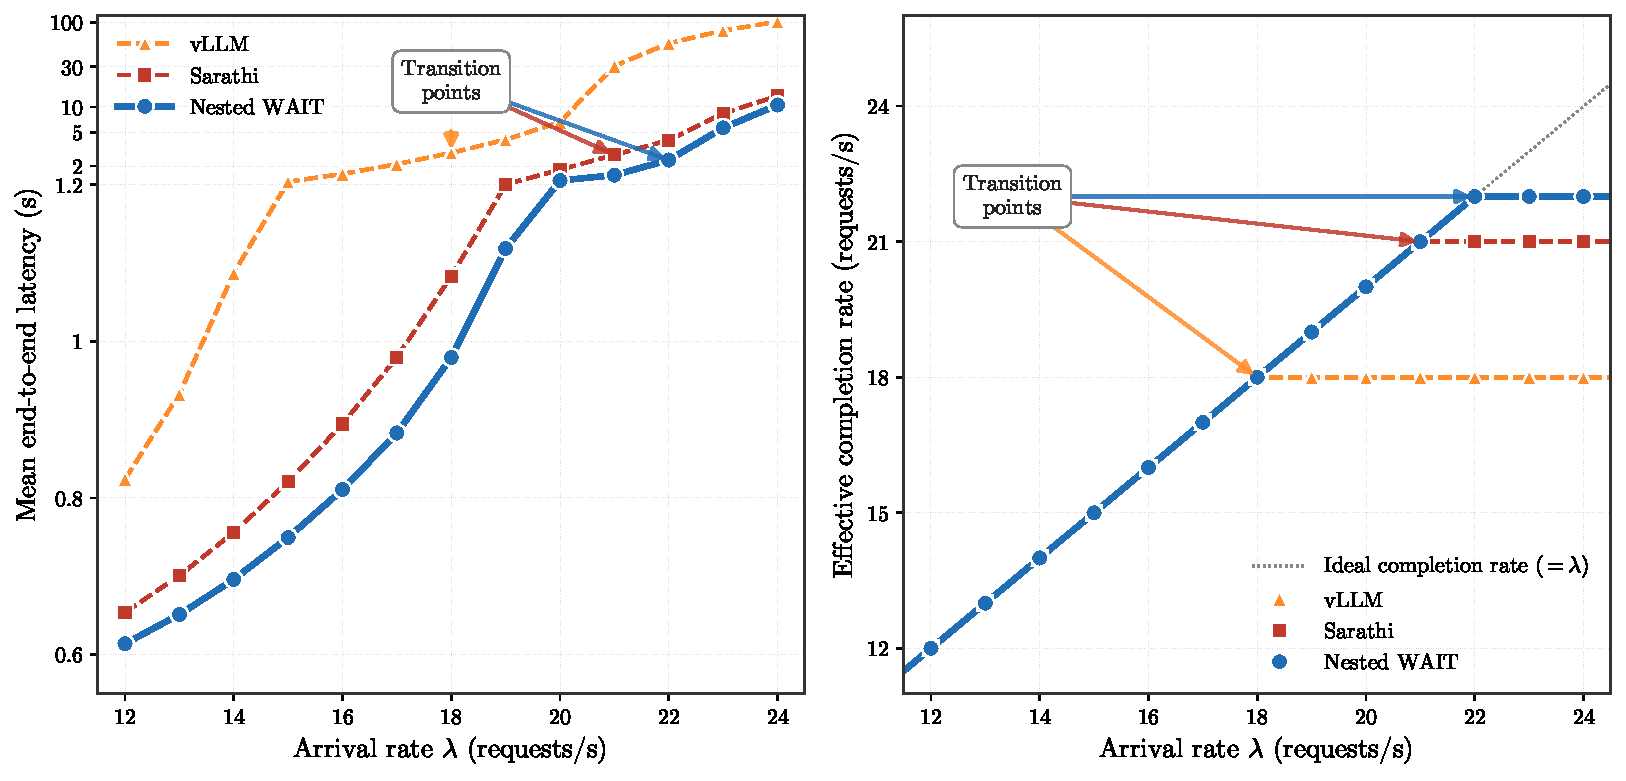
\includegraphics[width=0.76\textwidth]{Experiments_pdf/figure_C_multi_type.pdf}
    \caption{Two-type workload $(0.7\,\texttt{p512d20},\,0.3\,\texttt{p512d50})$: mean end-to-end latency (left) and effective completion rate (right) versus $\lambda$. The transition ordering is vLLM ($\hat{\lambda}^* = 18$), Sarathi ($\hat{\lambda}^* = 21$), and Nested WAIT ($\hat{\lambda}^* = 22$).}
    \label{fig:multi_type_rate}
\end{figure}

\paragraph{Long-decode regime.}
We also study the long-decode workload \texttt{p512d1000} with Poisson arrivals at $\lambda = 0.5, 1.0, \ldots, 5.0$. Relative to the single-type workload \texttt{p512d20}, each request now occupies about $30\times$ more KV cache, so all three policies lose stability at much smaller arrival rates. Figure~\ref{fig:long_decode} shows that at low rates $\lambda \leq 2.5$ the three policies are nearly indistinguishable, but near the boundary WAIT again has the lowest latency: at $\lambda = 4.5$ it attains $32.3$\,s versus $41.7$\,s for Sarathi and $53.8$\,s for vLLM. The intuition is that long-decode requests stay in the system for many more iterations, so excess admission persists longer and makes it harder to keep arrivals and completions in balance. WAIT performs better in this regime because it keeps the in-system inventory closer to that balance point. The same pattern is already visible at $\lambda = 4.0$, where the baseline-memory setting gives $26.4$\,s for WAIT versus $30.2$\,s for Sarathi. Table~\ref{tab:eviction} reports the accompanying eviction-induced restart evidence at the same arrival rate: Sarathi incurs a $2.88\%$ restart rate, whereas WAIT still avoids eviction altogether. Under the server's last-in-first-out eviction rule, each evicted request loses its partial decode progress and begins again from prefill, so the restart gap is another manifestation of the same imbalance.

\begin{figure}[htbp]
    \centering
    
\includegraphics[width=0.74\textwidth]{Experiments_pdf/figure_G_long_decode.pdf}
    \caption{Long-decode workload (\texttt{p512d1000}): mean end-to-end latency (left) and effective completion rate (right) versus $\lambda$. The main separation emerges from $\lambda \approx 3.0$ onward; near the boundary, WAIT attains the lowest latency and highest completion rate.}
    \label{fig:long_decode}
\end{figure}

\begin{table}[h]
\centering
\small
\begin{tabular}{lcc}
\toprule
Metric & Sarathi & WAIT (ours) \\
\midrule
Mean end-to-end latency ($\lambda = 4.0$) & $30.2$\,s & $26.4$\,s \\
Eviction-induced restart rate ($\lambda = 4.0$) & $2.88\%$ & $0\%$ \\
\bottomrule
\end{tabular}
\caption{Eviction diagnostic for \texttt{p512d1000} at $\lambda = 4.0$.}
\label{tab:eviction}
\end{table}

\paragraph{Long-horizon check near the transition.}
To check the estimated transition, we vary the simulation horizon at the two arrival rates nearest Nested WAIT's transition. Figure~\ref{fig:fin_horizon} plots mean latency on $(0.7\,\texttt{p512d20},\,0.3\,\texttt{p512d50})$ for $\lambda \in \{22, 23\}$ as $N$ increases from $2{,}000$ to $20{,}000$. At $\lambda = 22$, Nested WAIT approaches a finite latency plateau, whereas Sarathi's mean latency grows rapidly over the tested horizons. At $\lambda = 23$, both policies exhibit continued latency growth, but Nested WAIT remains $30\%$--$50\%$ below Sarathi at every horizon we consider. These comparisons are consistent with the observed transition from near-overloaded to overloaded operation lying between the two rates.

\begin{figure}[htbp]
    \centering
    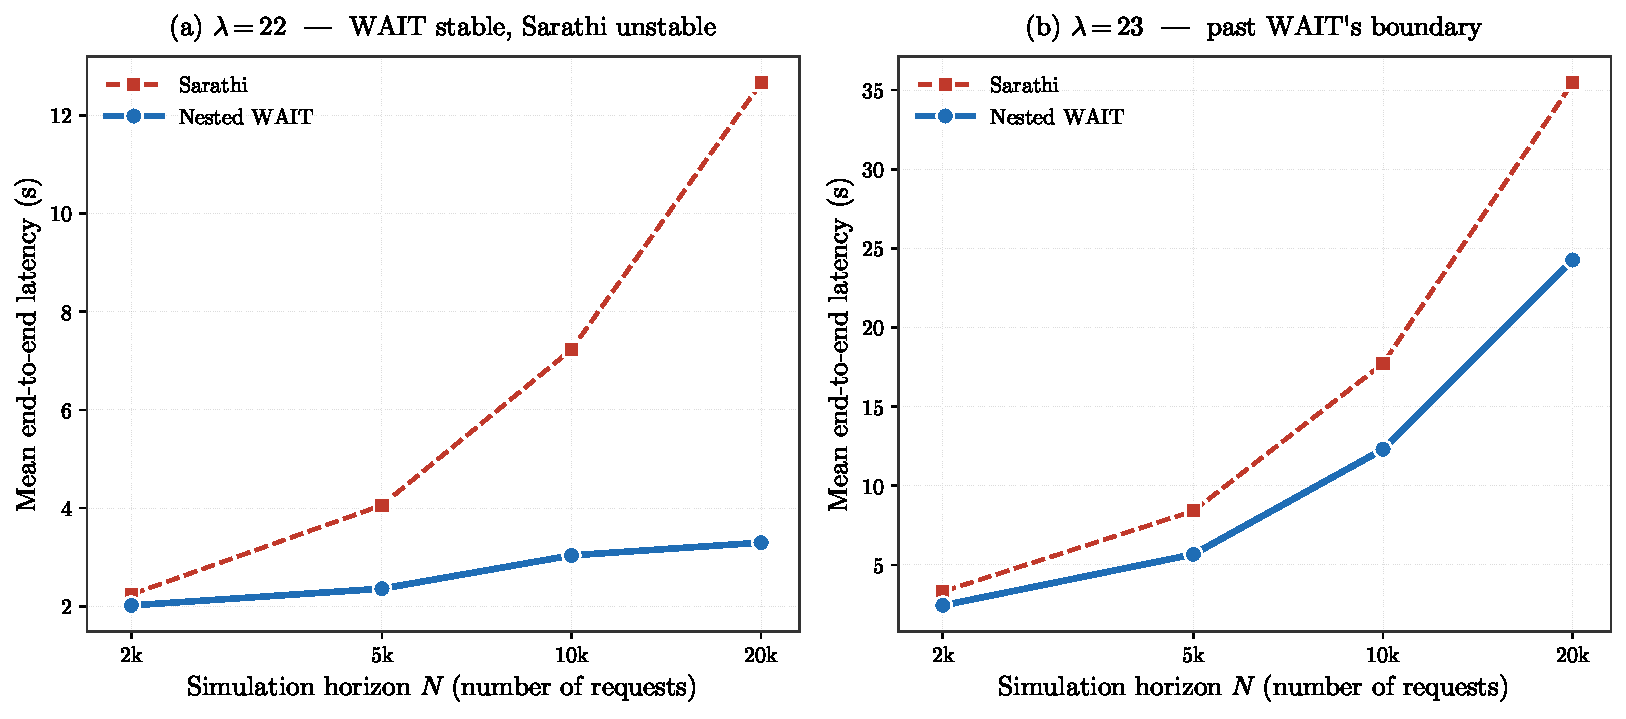
\includegraphics[width=0.76\textwidth]{Experiments_pdf/figure_E_stability.pdf}
    \caption{Long-horizon check near the transition on $(0.7\,\texttt{p512d20},\,0.3\,\texttt{p512d50})$. At $\lambda = 22$, Nested WAIT approaches a finite latency plateau; at $\lambda = 23$, both policies show continued latency growth, but Nested WAIT remains lower-latency.}
    \label{fig:fin_horizon}
\end{figure}

\subsection{Application to the \texttt{lmsys-chat-1m} Dataset}
\label{sec:exp_real}

We next evaluate the policies on \texttt{lmsys-chat-1m}, a real dataset with heterogeneous prompt and response lengths, where decode lengths are unknown at admission. This empirical setting lets us assess the robustness of Nested WAIT's state-dependent admission rule under a heterogeneous workload distribution, and characterize how the induced capacity allocation varies across prefill and decode stages.

\paragraph{Dataset.}
The dataset contains approximately $1$ million human--LLM conversations; we treat each user message as the prompt (prefill) and the corresponding assistant response as the generated output (decode). Figure~\ref{fig:lmsys_distribution} shows the prefill-length and decode-length distributions after filtering to requests with both lengths below $500$ tokens, which is the workload population used for sampling. Prefill lengths have mean $58.6$ tokens and median $21$, while decode lengths have mean $147.3$ tokens and median $116$. Short responses remain common: about $31\%$ of prompts decode for at most $50$ tokens, whereas about $14\%$ exceed $300$. For simulation, we sample $5{,}000$ requests from this filtered workload population. Arrivals follow a Poisson process with rate $\lambda$, measured in requests per second. All runs use the same simulator, hardware, and baseline settings as in Section~\ref{sec:exp_synthetic}.

\begin{figure}[ht]
    \centering
    
\includegraphics[width=0.66\textwidth]{Experiments_pdf/question_answer_lengths_distribution.pdf}
    \caption{Filtered \texttt{lmsys-chat-1m} prefill and decode length distributions. Dashed lines mark means and medians.}
    \label{fig:lmsys_distribution}
\end{figure}

\paragraph{Nested WAIT calibration on the real dataset.}
For the real-data runs, Nested WAIT applies the segment construction described above to the empirical decode-length distribution. The decode horizon \(0\)--\(500\) is divided into \(L\) equal-width segments, and a request is counted against the threshold of the segment containing its current decode stage. It first consumes capacity in the head segment and enters downstream segments only if it continues decoding, so the policy allocates admission capacity across realized continuation stages rather than making scheduling decisions from predicted final response lengths. All real-data arrival-rate runs use the baseline KV-cache cap of approximately \(1.37\times 10^5\) tokens described above. The cap \(\mathrm{tl}\) should not be read as allowing \(\mathrm{tl}\) longest-context requests to reside on the GPU simultaneously: resident KV-cache use depends on the realized prompt lengths and decode stages, and exceeding the memory cap triggers eviction and restart. In the experiments, we set \(\eta=0.05\), choose \(L\) from \(\{1,2,3,4,5,10,20\}\), and use the lowest-latency configuration on this parameter grid for each offered arrival rate. The performance is not monotone in either parameter: a cap that is too small leaves batching and downstream control underused, whereas a cap that is too large can push resident KV-cache usage toward overflow. Similarly, too few segments blur meaningful decode-stage differences, while too many segments fragment the segment-level caps and make prompts wait at segment thresholds too often. The selected setting is therefore the best tradeoff on this parameter grid for the workload and arrival rate.

To relate the real-data arrival rates to the fluid memory condition, Table~\ref{tab:lmsys_mstar} reports \(M^*(\lambda)\) for the same real-data sample. We compute these values by estimating the service-time parameters from our experiments and substituting the empirical prefill/decode length distribution into the fluid memory formula~\eqref{eq:memory_multi2}. The calculation places the fluid memory crossing \(M^*(\lambda)=C\) between \(\lambda=70\) and \(\lambda=80\), at approximately \(74.1\) queries/s. This is consistent with the range where the real-data latency and completion-rate curves begin moving from near-overloaded to overloaded operation; the remaining gap is expected from integer threshold rounding, finite-horizon stochastic variation, and the discrete segment calibration used by Nested WAIT.

\begin{table}[htbp]
\centering
\small
\begin{tabular}{rccc}
\toprule
Arrival rate \(\lambda\) & \(M^*(\lambda)\) (KV tokens) & \(M^*(\lambda)/C\) & Fluid stable region \\
\midrule
50 & \(34{,}377\)  & \(0.25\) & inside \\
60 & \(55{,}758\)  & \(0.41\) & inside \\
70 & \(100{,}327\) & \(0.73\) & inside \\
80 & \(250{,}509\) & \(1.83\) & outside \\
\bottomrule
\end{tabular}
\caption{Fluid memory requirement for the real dataset. The capacity is \(C\approx 1.37\times 10^5\) KV-cache tokens.}
\label{tab:lmsys_mstar}
\end{table}

\paragraph{Results.}
Figure~\ref{fig:lmsys_rate} varies the arrival rate $\lambda$ from $10$ to $150$ in steps of $10$. The plotted comparison follows the same qualitative ordering as the synthetic experiments. The baseline schedulers are competitive when the workload is light, but their latencies increase more quickly as the system approaches and then exceeds the range in which completions can keep pace with arrivals. Nested WAIT is most clearly separated from the baselines in these near-overloaded and overloaded regimes. This pattern is consistent with the heterogeneous decode distribution: many requests finish in the early decode stages, while a smaller group remains active for hundreds of generated tokens. Nested WAIT's nested thresholds control how many requests may continue across successive decode-stage ranges, allowing short responses to clear early while limiting the population in later decode stages that consumes KV-cache capacity.

\begin{figure}[htbp]
    \centering
    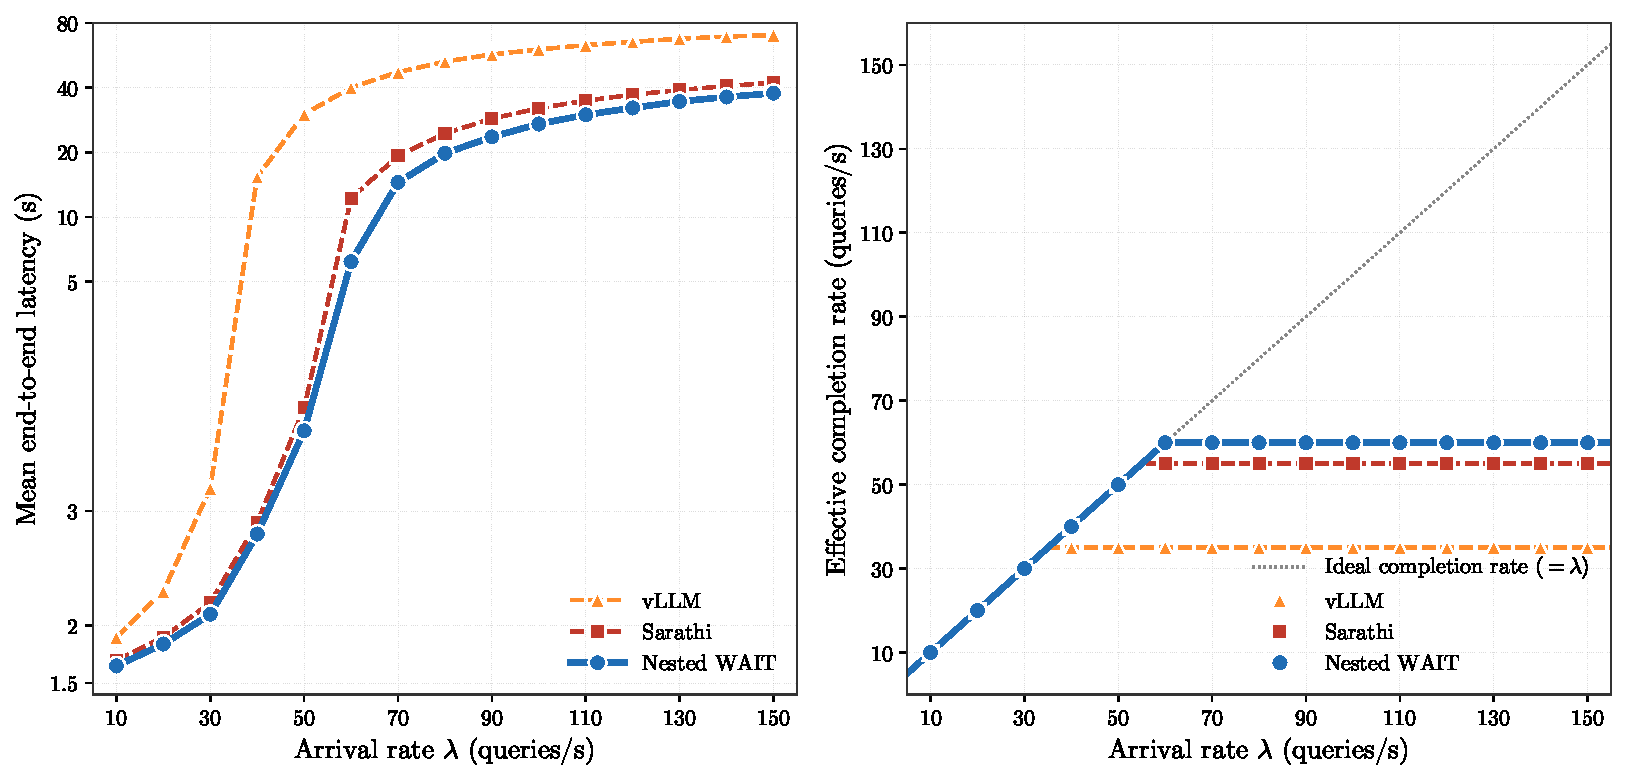
\includegraphics[width=0.68\textwidth]{Experiments_pdf/figure_D_lmsys_real.pdf}
    \caption{Real-data experiment on \texttt{lmsys-chat-1m} ($5{,}000$ requests): mean end-to-end latency (left) and effective completion rate (right) versus $\lambda$. Nested WAIT has a larger latency gap near overload.}
    \label{fig:lmsys_rate}
\end{figure}
